\documentclass[a4paper,11pt]{article}
\usepackage[big]{layaureo}
\usepackage[T1]{fontenc}
\usepackage[utf8]{inputenc}
%\usepackage[italian]{babel}
\usepackage{fancyhdr}
\usepackage{textcomp}
\usepackage{amsmath}
\usepackage{amssymb}
\usepackage{mathtools}
\usepackage{multirow}
\usepackage{caption}
  \captionsetup{format=plain,labelfont=bf,textfont=it, font=small}
\usepackage{subcaption}
  \captionsetup[sub]{position=top}
  \captionsetup[sub]{font=footnotesize}
  \captionsetup[sub]{labelfont={bf,sc}}
  \captionsetup[sub]{format=hang}
\usepackage{booktabs}
\usepackage{tabularx}
\usepackage{float}
\usepackage{wrapfig}
\usepackage{comment}
\usepackage[dvipsnames]{xcolor}
\usepackage{listings}
\definecolor{light-gray}{gray}{.95}
\lstset{frame=none,
  aboveskip=3mm,
  belowskip=3mm,
  showstringspaces=false,
  columns=fullflexible,
  keepspaces=true,
  numbers=none,
  basicstyle={\footnotesize\ttfamily},
  numberstyle=\tiny\color{gray},
  keywordstyle=\color{NavyBlue},
  stringstyle=\color{Orange},
  commentstyle=\color{OliveGreen},
  breaklines=true,
  breakatwhitespace=true,
  tabsize=4,
  backgroundcolor=\color{light-gray}
}

\title{Neural Network and Deep Learning \\ Homework 4}
\author{Federico Agostini}
\date{}

\begin{document}

\maketitle

\section{Introduction}
In this exercise unsupervised learning is explored using autoencoders on the MNIST dataset. Hyperparameters are optimized; in particular a sistematic serch over the size of the hidden layer is done. The trained model is then tested on both original images and corrupted versions.

\section{Parameters tuning}

Tuning process is done in two separate phases; in the first one the optimizer is tuned, and then the influence of the size of the hiddeen layer is explored. The same network architecture proposed during the laboratory is used.

The optimizer chosen is Adam; in order to tune the learning rate and weight decay (L2 penalty), a grid search with cross validation with 3 folds is implemeted with 20 training epoches. Learning rate values are \texttt{[5e-02, 1e-02, 5e-03, 1e-03, 5e-04, 1e-04]}, while the weight decay spans in the list \texttt{[5e-04, 1e-04, 5e-05, 1e-05, 5e-06, 1e-06]}. Only the training set is used in this phase. Best combinations of parameters with respect to the validation loss (MSE) are shown in Tab.~\ref{tab:opt_loss}.

\begin{table}[hp]
  \centering
  \caption{Best values for the learning rate and weight decay of the Adam optimizer.}
  \label{tab:opt_loss}
  \begin{tabular}{cccc}
    \toprule
      Learning rate & Weight decay &  Train Loss &  Validation Loss \\
    \midrule
      0.0100 &  0.000005 &    0.021793 &  0.022443 \\
      0.0100 &  0.000010 &    0.022037 &  0.022501 \\
      0.0050 &  0.000005 &    0.022173 &  0.022681 \\
      0.0050 &  0.000010 &    0.022197 &  0.022696 \\
      0.0050 &  0.000050 &    0.023330 &  0.023907 \\
    \bottomrule
    \end{tabular}
\end{table}

Fixed those hyperparameters, another search over the size of the hidden layer is done. In this case, the whole training set is used for training, while the loss is estimated with the test set (the mean value of the last 5 epoches is used). In order to avoid overfitting, a scheduler is also added to reduce the learning rate in case the test loss does not decrease for 5 consecutive iterations (\texttt{ReduceLROnPlateau} on Pytorch). The number of training epoches is now set to 50. Fig.~\ref{fig:hidden_loss} shows the test loss for different size of the hidden layer, while Tab.~\ref{tab:esd} has the numerical values of the final loss. The best model results to be the one with an embedding dimension of 20 and Fig.~\ref{fig:train-test_loss} represents its training and test loss as function of the epoch.

\begin{figure}[htp]
  \centering
  \caption{}
  \begin{subfigure}[t]{.45\linewidth}
    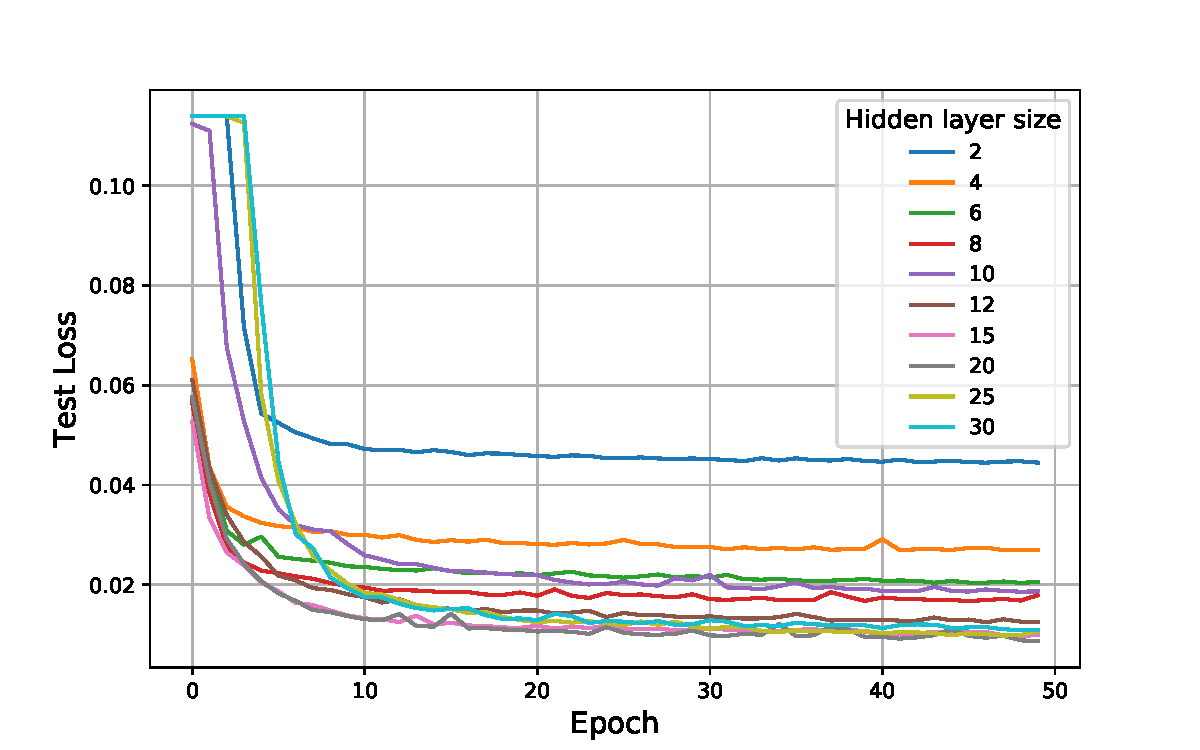
\includegraphics[width=\linewidth]{../hidden_loss.pdf}
    \caption{Test loss for different size of the hidden layer.}
    \label{fig:hidden_loss}
  \end{subfigure}
  \begin{subfigure}[t]{.45\linewidth}
    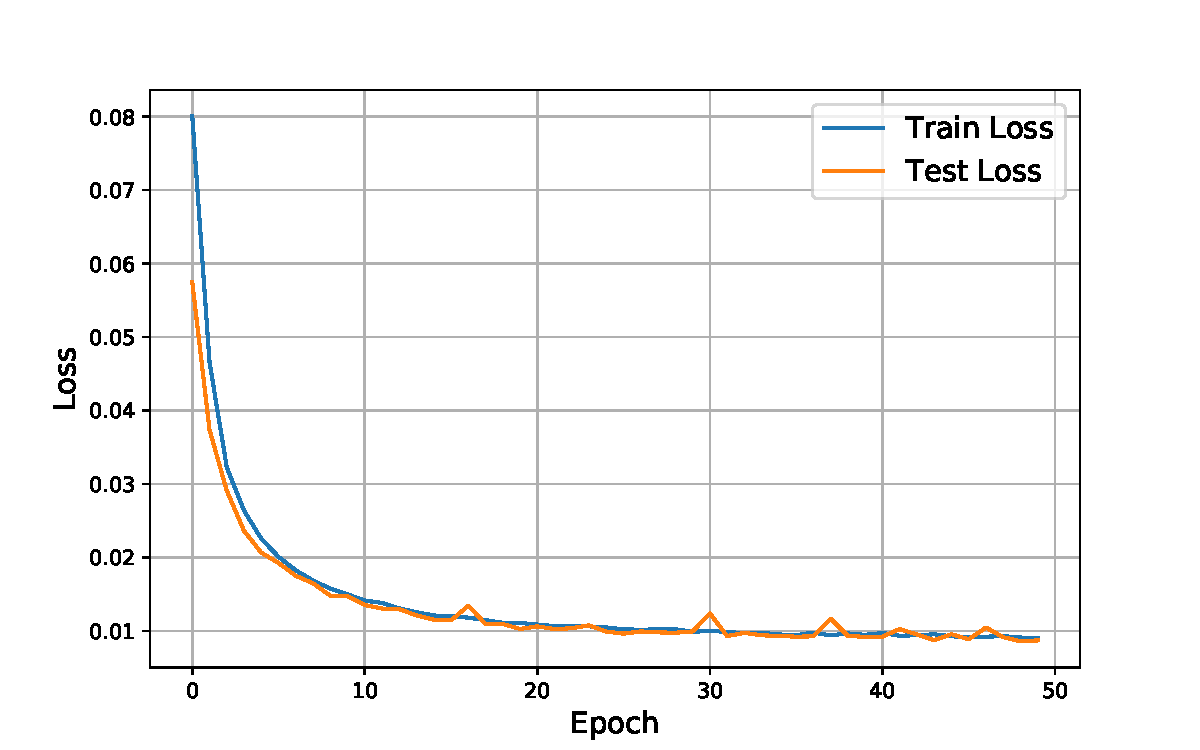
\includegraphics[width=\linewidth]{../train-test_loss_best.pdf}
    \caption{Train and test loss for the best model (embedding space dimension equal to 20).}
    \label{fig:train-test_loss}
  \end{subfigure}
\end{figure}

\begin{table}
  \centering
  \caption{Test loss as function of the size of the embedding layer.}
  \label{tab:esd}
  \begin{tabular}{cc|cc}
    \toprule
    Size &  Test Loss & Size &  Test Loss \\
    \midrule
     20 &   0.009258 & 8  &   0.017079\\
     15 &   0.010073 & 10 &   0.018720\\
     25 &   0.010108 & 6  &   0.020458\\
     30 &   0.011145 & 4  &   0.027136\\
     12 &   0.012720 & 2  &   0.044586\\
    \bottomrule
  \end{tabular}
\end{table}

\section{Reconstruction capability}
The trained final model with 20 as encoded space dimension is then tested. On the MNIST test set the MSE is 0.0086. Images are the corrupted either adding normal noise or deleting a portion of the image itself.

\paragraph{Noise} Noise applied is proportional to $\mathcal{N}(0,1)$, with a prefactor $\alpha \in [0,1]$. Fig.~\ref{fig:noise} represents the MSE loss as function of the noise level, along with an example of the reconstructed image of the autoencoder.

\begin{figure}[htp]
  \centering
  \caption{MSE loss as function of the noise level and example of the autoencoder reconstruction.}
  \label{fig:noise}
  \begin{subfigure}[c]{.45\linewidth}
    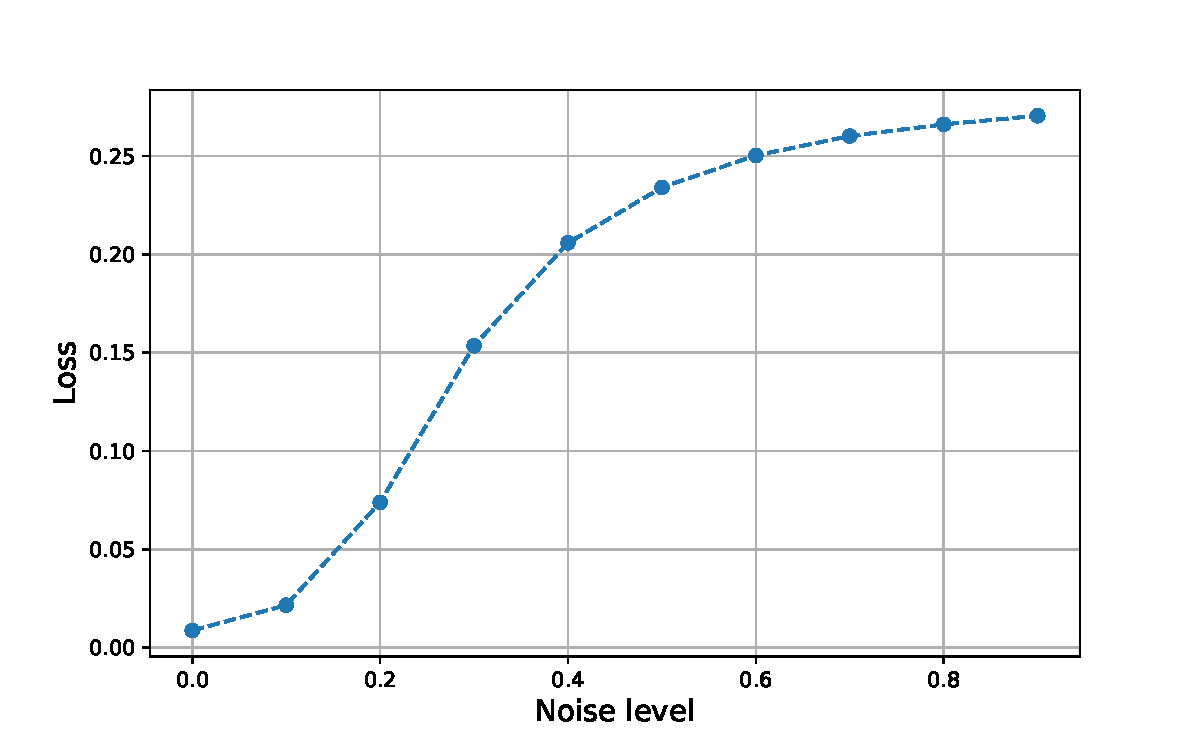
\includegraphics[width=\linewidth]{../noise/loss.pdf}
  \end{subfigure}
  \begin{subfigure}[c]{.45\linewidth}
    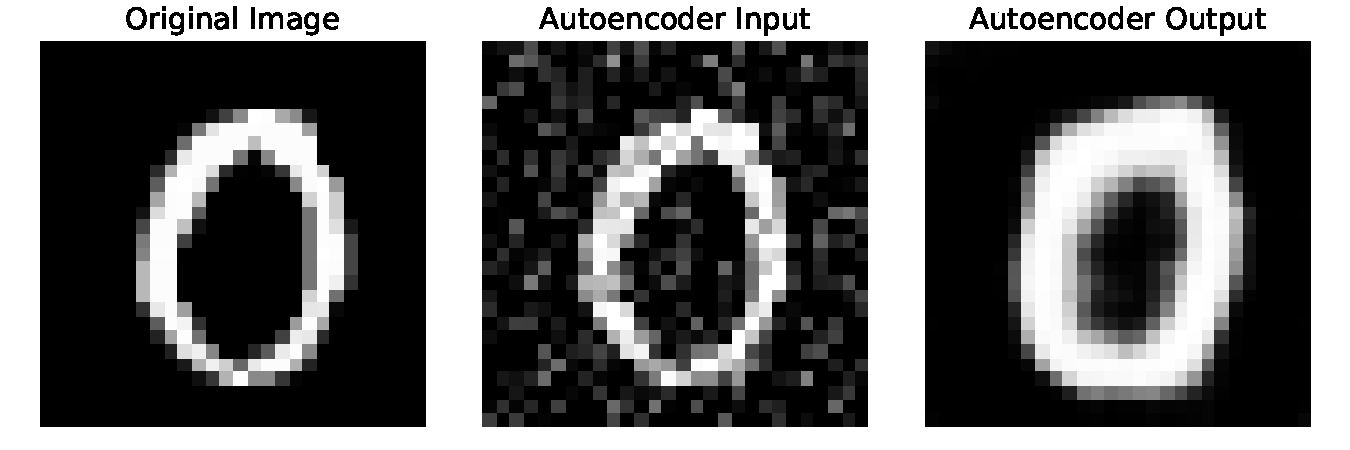
\includegraphics[width=\linewidth]{../noise/02.pdf}
  \end{subfigure}
\end{figure}

\paragraph{Occlusion} The occlusion level represents the fraction of pixel deleted. Fig.~\ref{fig:occlusion} shows the MSE loss as function of the occlusion level along with an example of a reconstructed image.

\begin{figure}[htp]
  \centering
  \caption{MSE loss as function of the occlusion level and example of the autoencoder reconstruction.}
  \label{fig:occlusion}
  \begin{subfigure}[c]{.45\linewidth}
    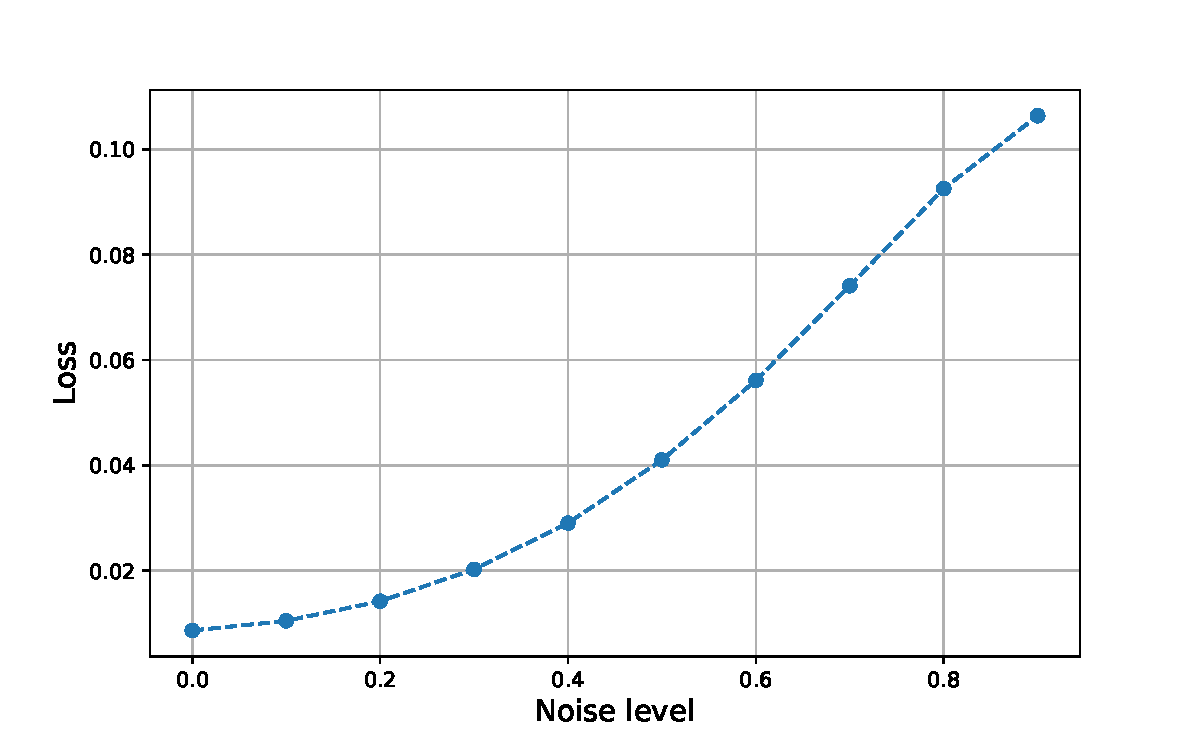
\includegraphics[width=\linewidth]{../occlusion/loss.pdf}
  \end{subfigure}
  \begin{subfigure}[c]{.45\linewidth}
    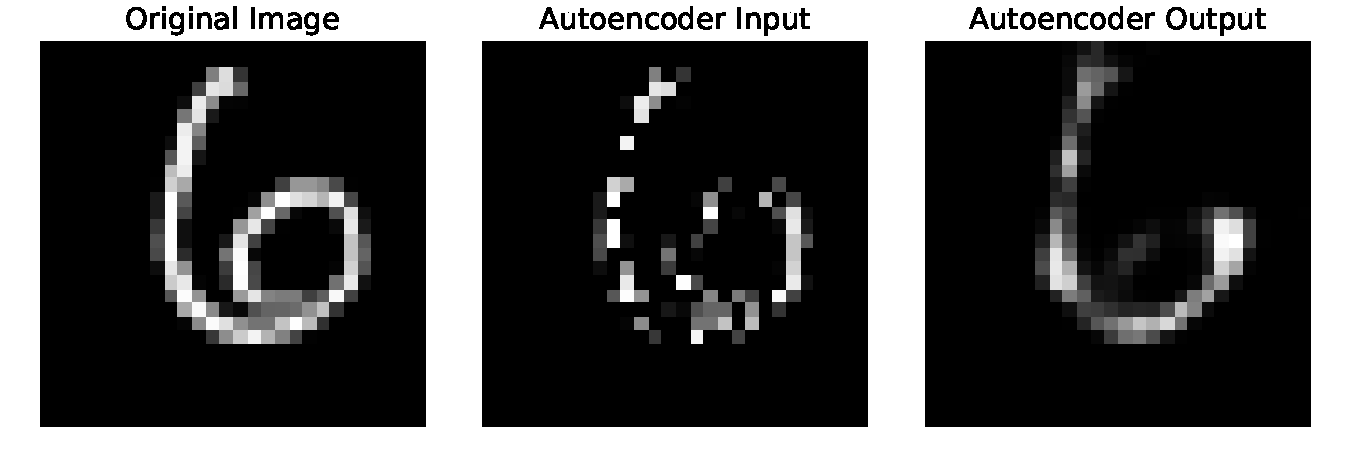
\includegraphics[width=\linewidth]{../occlusion/05.pdf}
  \end{subfigure}
\end{figure}

\section{Encoding space}
The representational space of the best model has dimension 20; in order to visualize it in 2 dimensions, t-SNE is used. Fig.~\ref{fig:tsne} shows how different digits are grouped in the encoding space (2000 samples are plotted). It can be noticed that different digits clearly form separated clusters, so nearby points in the encoding space produce similar images.

\begin{figure}[htp]
  \centering
  \caption{Encoding space visualization using t-SNE to reduce the dimensionality from 20 to 2.}
  \label{fig:tsne}
  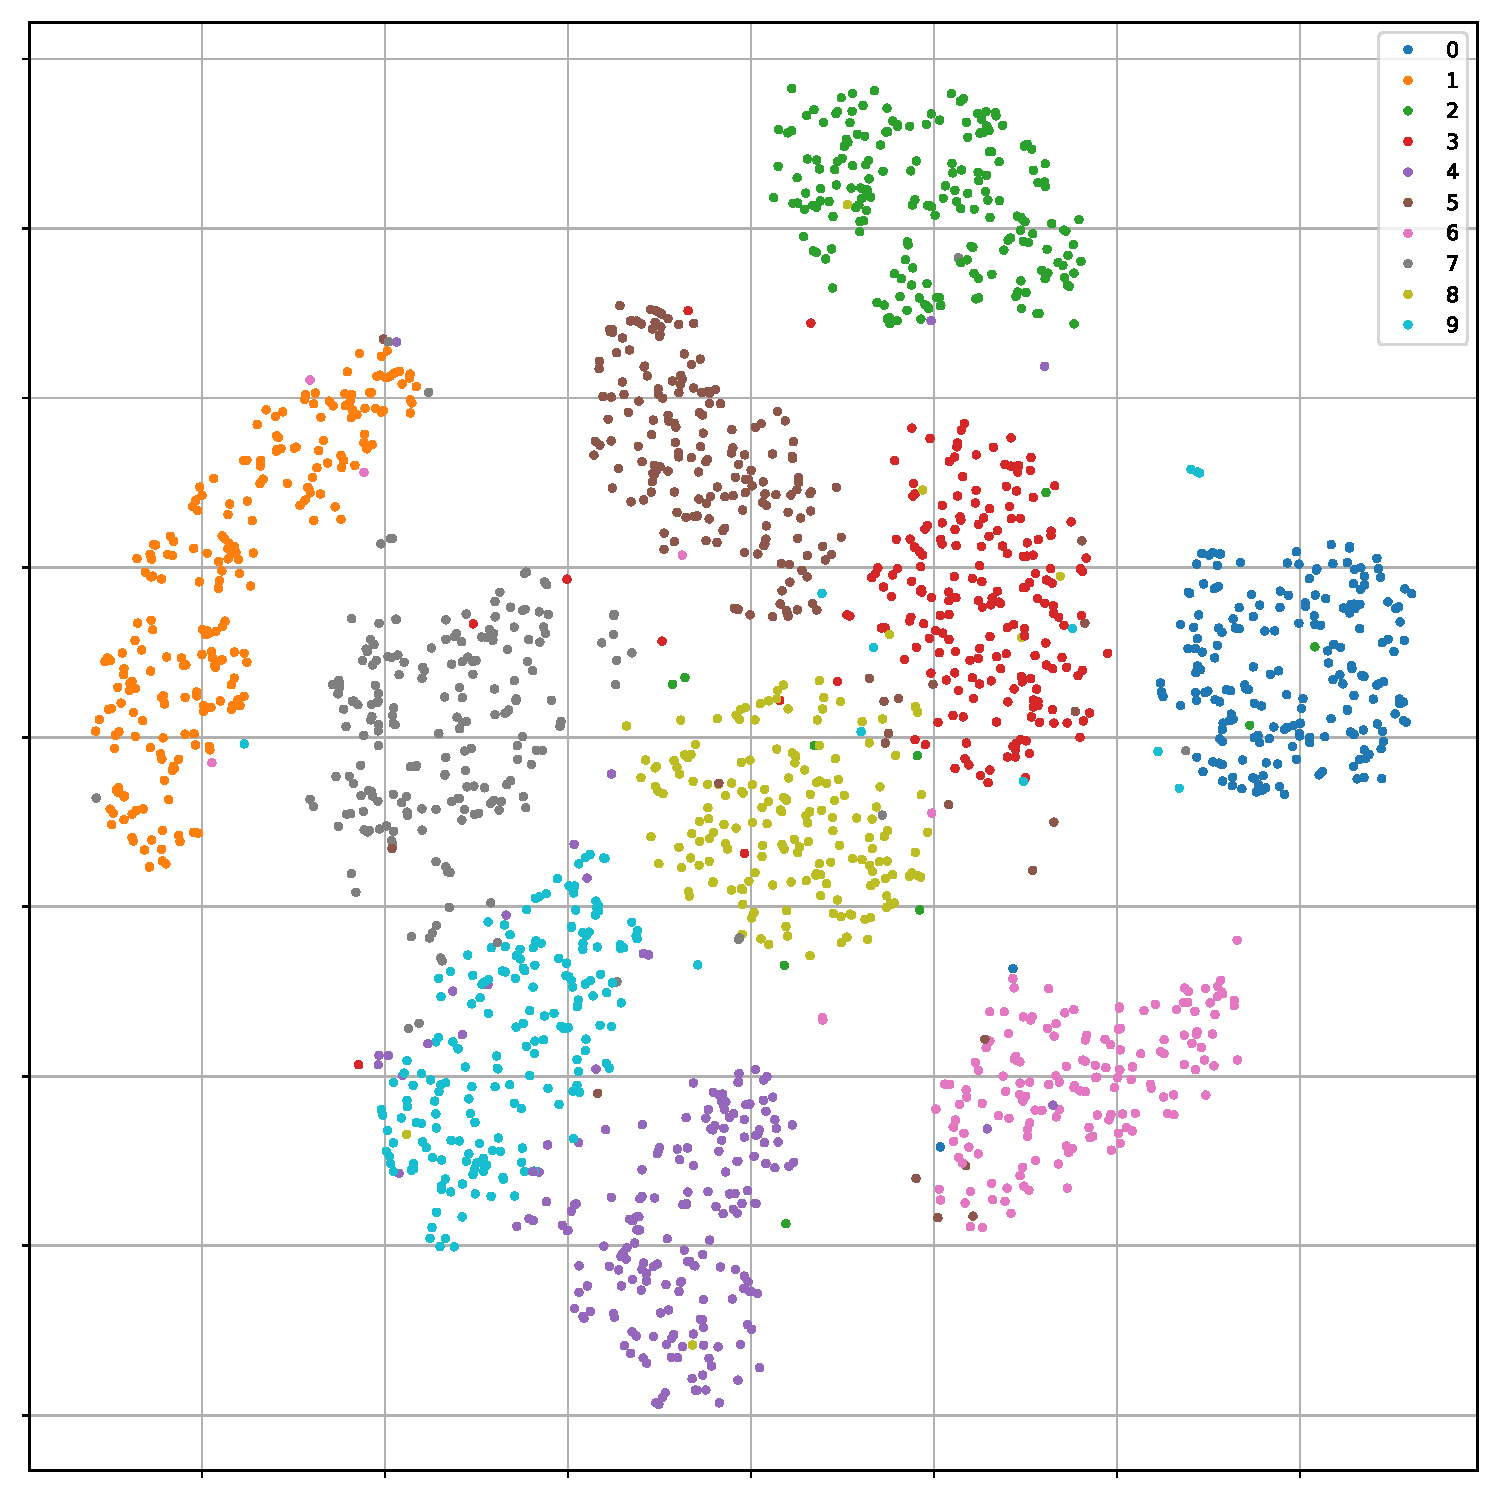
\includegraphics[scale=.5]{../encoded_space.pdf}
\end{figure}

\end{document}
